\chapter{MODELOS OCULTOS DE MARKOV}
\thispagestyle{plain}
\label{chap:hmm}
Neste capítulo é realizada a descrição do algoritmo HMM. A seção \ref{sec:topo} traz uma análise das diferentes topologias do HMM e a seção \ref{sec:3prob} mostra os três problemas a serem solucionados no algoritmo.

\quad Um modelo de Markov pode ser definido como um conjunto finito de estados ligados entre si por transições, formando uma máquina de estados. Estas transições estão ligadas por um processo estocástico .  Há ainda um outro processo estocástico associado a um modelo de Markov, que envolve as observações de saída de cada estado. Se somente as observações de saída forem visíveis a um observador externo ao processo, diz-se então que os estados estão ocultos. %, ou seja, o processo estocástico que envolve as transições de estado não é observavel.( aparentemente por isso que é oculto)

%De forma simplificada, podemos dizer que processos estocásticos são processos aleatórios que dependem do tempo. ; Um processo estocástico é uma família de variáveis aleatórias indexadas por elementos t pertencentes a determinado intervalo temporal.Wipedia acho.).

Um HMM é caracterizado por:
\begin{itemize}

\item  Um conjunto de estados $ S =  \{S_1, S_2, \ldots, S_{n-1}, S_n\} $, onde $n$ é o número de estados;

\item Função de probabilidade de estado inicial $\pi = \{\pi_i\}$ .

\begin{equation}
\pi_i = P[q_1 = S_i ]~~\textrm{ }~ 1 \leq i \leq n 
\end{equation}
onde $q_1$ é o estado inicial $(t = 1)$.

\item Função de probabilidade de transição A;

\item Função de probabilidade de símbolos de saída B.

\end{itemize}

Considerando exclusivamente processos em que as probabilidades de transição não dependem do tempo e os HMMs são de primeira ordem, um HMM é considerado de primeira ordem quando a trasição do estado depende apenas da probabilidade do estado anterior mais recente. O conjunto de probabilidades de transição $A$ é definido por: 
 \begin{equation}
A = \{ a_{ij}\} 
\end{equation}

 \begin{equation}
 a_{ij} =  P [q_{t-1} = S_i] [q_t = S_j]~~\textrm{ }~ 1 \leq i, j\leq n
\end{equation}

onde $a_{ij}$ é a probabilidade de ocorrer uma transição do estado $S_i$ para o estado $S_j$.\\
Os coeficientes $a_{ij}$ devem obedecer às seguintes regras:

\begin{equation}
a_{ij} \geq 0~~\textrm{ }~ 1 \leq i,j \leq n 
\end{equation}

\begin{equation}
\displaystyle \sum_{j=1}^n a_{ij} = 1~\textrm{ }~ 1 \leq i \leq n 
\end{equation}

A probabilidade de estar no estado $S_j$ no instante de tempo $t$ depende somente do instante de tempo $t_j$.\\

\section{HMM e a função densidade de probabilidade}
\quad Um HMM também pode ser classificado de acordo com a função densidade de probabilidade. 

\subsection{Função densidade de probabilidade}
\quad Uma variável aleatória é uma função cujo valor é um número real determinado por cada elemento em um espaço amostral. Dada uma variável aleatória $X$, dizemos que $f(x)$ é uma função densidade de probabilidade de $X$, se e somente se $f(x)$ atender as seguintes condições:

$$
\displaystyle f(x) \geq 0  \qquad a < x < b
$$

\begin{equation}
 \int_a^b f(x)dx = 1 
\end{equation}

\subsection{HMM Discreto}
\quad O número de possíveis símbolos de saída é finito \cite{fundRecFala}.
 A probabilidade de emitir o símbolo $V_k$ no estado $S_i$ é dada por $b_i(k)$. As propriedades da função de probabilidade $B$ são:

$$
 \displaystyle  b_i (k) \geq 0 \qquad 1 \leq i \leq n  \qquad 1 \leq k \leq K
$$

\begin{equation}
\displaystyle \sum_{k=1}^K b_i (k) = 1 \qquad 1 \leq i \leq n 
\end{equation}

As observações são discretas por natureza ou discretizadas através de uma técnica de quantização vetorial, gerando assim \textit {codebooks}.
 
\subsection{HMM Contínuo}
\quad A função densidade de probabilidade é contínua. Geralmente uma função densidade elipticamente simétrica, tal como a função densidade de probabilidade Gaussiana \cite{fundRecFala}.
 As observações são contínuas e a FDP contínua é  usualmente modelada como uma mistura finita de matrizes gaussianas multidimensionais.
% DEFINIR AQUI A FDP A SER USADA (PROVAVELMENTE A GAUSSIANA CITADA EM  \cite{fundRecFala})
\subsection{HMM Semicontínuo}
\quad O modelo é um caso intermediário entre contínuo e o discreto. O conjunto função densidade probabilidade é o mesmo usado para todos os estados e todos os modelos. A probabilidade de emissão dos símbolos de saída é dada por :


\begin{equation}
\displaystyle b_j(O_t) =  \sum_{V_k \in \eta (O_t)}^-  c_j (k) f (O_t | V_k)   \qquad 1 \leq j \leq n 
\end{equation}
 onde:\\
$O_t$ é o vetor de entrada\\
$\eta(O_t)$ é o conjunto das funções densidade de probabilidade que apresentam os $M$ maiores valores de $f (O_t | V_k)$, $ 1 \leq M \leq K$\\
$K$ é o número de funções densidade de probabilidade, ou seja, os símbolos de saída\\
$V_k$ é o $k$-ésimo símbolo de saída\\
$ c_j (k)$ é a probabilidade de emissão do símbolo $V_k$ no estado $S_j$\\
$f (O_t | V_k)$ é o valor da $k$-ésima função densidade de probabilidade.



\section{Topologia}
\label{sec:topo}

\quad Uma maneira de classificar um HMM é de acordo com a estrutura de transição da matriz $A$ da cadeia de markov. Existem vários modelos de HMM, a Figura \ref{fig:topohmm} ilustra os  principais modelos de acordo com \cite{fundRecFala}. O ergódico totalmente conectado onde qualquer estado pode ser alcançado com um único passo, o modelo de caminhos paralelos e o modelo "left-right", também chamado de modelo Bakis.%\\ *********COLOCAR AQUI UM MODELO DE BAKIS FAZER A MATRIZ
\begin{figure}[H]
\centering % para centralizarmos a figura
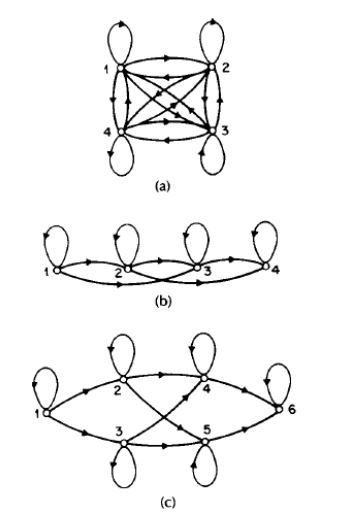
\includegraphics[width=10cm]{img/topohmm.jpg} % leia abaixo
\caption{Exemplo de topologias de HMM. a) Modelo ergódico b) Modelo esquerda-direita c) Modelo esquerda-direita paralelo. \textit{\cite{fundRecFala}}}
\label{fig:topohmm}
\end{figure}

\section{Os problemas a serem resolvidos}
\label{sec:3prob}
\quad O HMM possui três problemas básicos, que são:
\begin{enumerate}
\item \textbf{Problema de avaliação:} Dada a sequência de observação $O = (o_1, o_2, o_3, ..., o_n)$ e o modelo $\lambda = (A, B, \pi)$, como calcular eficientemente $P(o| \lambda)$.
\item \textbf{Problema da busca da melhor sequência de estados.}
\item \textbf{Problema de treinamento:} como ajustar os parâmetros do modelo $\lambda(A, B, \pi)$ para maximizar $P(o|\lambda)$.
\end{enumerate}

O problema 1, ou seja, o problema da avaliação pode ser solucionado através do procedimento \textit{Forward-Backward}. O segundo problema é solucionado com a aplicação do algoritmo de \textit{Viterbi} e o terceiro e último problema pode ser otimizado aplicando um procedimento iterativo como o método de \textit{Baum-Welch}. Nas seções \ref{secFB}, \ref{secViterbi} e \ref{secBW} faz-se uma explicação sobre os procedimentos para a solução dos problemas 1, 2 e 3 respectivamente.

\subsection{Foward-Backward}
\label{secFB}
Com a resolução do problema 1 podemos responder à algumas perguntas, se dado um modelo e uma sequência de observações, como podemos  saber de que a sequência observada foi produzido pelo modelo? ou, podemos ver essa  solução de outra forma,  um modelo é satisfatório para determinada entrada de observações?
 \begin{itemize}
\item Inicialização:\\
\begin{equation}
\displaystyle  \alpha_1 (i) = \pi_i b_i (O_1), \qquad 1 \leq i \leq N \\
\end{equation}

\item Indução:\\
$
\displaystyle \alpha_t + 1 (j) = \sum\limits_{ i = 1}^{N} \Big[\alpha_t(i) a_{ij} \Big]b_j (O_t + 1), \qquad 2 \leq t \leq T\\
%\displaystyle \Psi_t (j) = arg\max\limits_{1 \leq i \leq N}\Big[\delta_{t-1} (i)a_{ij}\Big], \qquad 1\leq j \leq N
$

\item Término:\\
$
P(O| \lambda) =  \sum\limits_{ i = 1}^{N} \Big[\alpha_t(i) \Big]\\
$

\end{itemize}

\subsection{Viterbi}
\label{secViterbi}
O algoritmo de Viterbi é um algoritmo de programação dinâmica usado para encontrar a sequência de estados ocultos ótima. Dado uma sequência de estados ocultos de um HMM, o algoritmo de viterbi calcula a melhor sequência de estados baseados nas probabilidades de transição. Este algoritmo foi proposto em 1967 por Andrew Viterbi para a decodificação de códigos convolucionais em links de comunicação ruidosos.  O algoritmo também possui aplicações  em redes CDMA e GSM, modem dial-up, satélites, síntese de fala, linguística computacional e bioinformática. Em telecomunicação, um código convolucional é um tipo de código corretor de erro em que cada conjunto de $m$ símbolos é transformado em um conjunto de $n$ símbolos.\\
Algoritmo
\begin{itemize}
\item Inicialização:\\
\begin{equation}
\delta_1 (i) = \pi_i b_i (O_1), \qquad 1 \leq i \leq N \\
\end{equation}
$
\quad \Psi_1 (i) = 0
$

\item Recursão:\\
\begin{equation}
\displaystyle \delta_t (j) = \max\limits_{1 \leq i \leq N} \Big[\delta_{t-1}(i) a_{ij} \Big]b_j (O_t), \qquad 2 \leq t \leq T\\
\end{equation}
\begin{equation}
\displaystyle \Psi_t (j) = arg\max\limits_{1 \leq i \leq N}\Big[\delta_{t-1} (i)a_{ij}\Big], \qquad 1\leq j \leq N
\end{equation}

\item Término:\\
\begin{equation}
\displaystyle P^* =\max\limits_{1 \leq i \leq N}  \Big[\delta_{T(i)}\Big] 
\end{equation}
\begin{equation}
\displaystyle G^*_T = arg\max\limits_{1 \leq i \leq N}  \Big[\delta_{T(i)}\Big]
\end{equation}


\end{itemize}





\subsection{Baum-Welch}
\label{secBW}
Não existe uma maneira conhecida de resolver analiticamente o conjunto de parâmetros para um dado modelo de forma que seja maximizada a probabilidade da seqüência de observações. No entanto um procediemento iterativo como o método de Baum-Welch  permite escolher $\lambda = (A, B, \pi)$ tal que $P(O|\lambda)$ é maximizada localmente. O algoritmo Baum-Welch é apresentado em termos das variáveis $\alpha_t$ e $\beta_t$ dos algoritmos \textit {forward} e \textit{backward} respectivamente, e segundo  \cite{artRabiner} é o mais indicado para a estimação dos parâmetros do HMM. A re-estimação dos parâmetros $a_{ij}$ e $b_{ij}$ para uma dada sequência de observações através do método de Baum-Welch é descrita da seguinte forma por [19].\\
Para uma única sequência de observações $O = {O_1, O_2, \ldots, O_T}$ a re-estimação da probabilidade de transição do estado $i$ para o estado $j$ da matriz de transição de estados $A$ é dada por:


\begin{equation}
\displaystyle a_{ij} = \frac{\sum_{t=1}^{T-1} a_t(i)a_{ij}b_j (O_{t+1}) \beta_{t+1}(j)}{\sum_{t=1}^{T-1} a_t(i)\beta_t(j)}
\end{equation}


Para os HMM’s discretos, a quantidade de símbolos de saída é finita. Também para uma
única elocução, a re-estimação da função de probabilidade para que um estado $q_i$ emita um símbolo $O_t = V_k $ é obtida por:

\begin{equation}
\displaystyle  b_i(k) = \frac{\sum_{t=1}^{T-1} a_t(i)\beta_t(j) t.q. \quad O_t = V_k}{\sum_{t=1}^{T-1} a_t(i)\beta_t(j)}
\end{equation}

onde $ \displaystyle \qquad b_i(k) \geq 0, \qquad 1\leq i \leq N, \qquad 1 \leq k \leq M, \qquad \sum_{k=1}^M b_i(k) = 1, \qquad 1 \leq i \leq N$














